
\graphicspath{ {./figures/clones/} }

%CONTRIBUTIONS
%%%%%%%%%%%%%%%%%%%%%%%%%%%%%%%%%%%

\chapter{Automated analysis of mosaic eye imaginal discs in \textit{Drosophila}}
\label{ch:clones}

A manuscript closely resembling this chapter is currently in preparation for submission to a peer reviewed journal. The work was coauthored with Neda Bagheri and Lu\'{i}s Amaral, using experimental data borrowed from Nicol\'{a}s Pel\'{a}ez. These data are part of a larger study discussed at length in Chapter \ref{ch:ratio}.

%MANUSCRIPT
%%%%%%%%%%%%%%%%%%%%%%%%%%%%%%%%%%%

\section{Introduction}

Quantification will be essential as biologists study increasingly complex facets of organismal development \cite{Oates2009}. Unfortunately, qualitative analysis remains common because it is often difficult to measure cellular processes in their native context. Modern fluorescent probes and microscopy techniques make such measurements possible \cite{Muzzey2009a,Stelzer2014,Truong2011}, but the ensuing image analysis demands specialized skills that fall beyond the expertise of most experimentalists. Automated analysis strategies have addressed similar challenges in cytometry \cite{Aghaeepour2013,Chen2015,Pyne2009}, genomics and transcriptomics \cite{Bernstein2008,Hellemans2007,Langmead2012,Trapnell2009}, and other subdisciplines of biology \cite{Costes2004,Kelley2015}. Image analysis has proven particularly amenable to automation, with several computer vision tools having gained traction among biologists \cite{Carpenter2006,Paintdakhi2016,Schindelin2012,Sommer2011}. These platforms are popular because they increase productivity, improve the consistency and sensitivity of measurements, and obviate the need for specialized computational proficiency \cite{Jug2014,Sbalzarini2016,Schindelin2015}. Designing similar tools to help biologists probe and measure developmental processes in vivo will further transform studies of embryogenesis and development into quantitative endeavors.

Developmental biologists study how the expression and function of individual genes coordinate the emergence of adult phenotypes. They often ask how cells respond when a specific gene is perturbed during a particular stage of development. Cell response may be characterized by changes in morphology, or by changes in the expression of other genes (Fig. \ref{fig:clones:fig1}A). Experimental efforts to answer this question were historically stifled by the difficulty of isolating perturbations to a single developmental context, as the most interesting perturbation targets often confer pleiotropic function across several stages of development \cite{IanSimpson2002,Parody1993,Shilo1991}. 

Mosaic analysis addressed this challenge in \textit{Drosophila} by limiting perturbations to a subset of cells within the larval eye \cite{Xu1993,Xu2012}, a model system with enduring relevance \cite{Beira2016}. The technique yields a heterogeneous tissue comprised of genetically distinct patches of cells, or clones. Clone formation may be restricted to specific developmental contexts by using endogenously-activated promoters to drive trans-chromosomal recombination events \cite{Newsome2000,Theodosiou1998}. The timing of these events determines the number and size of the resultant clones \cite{Struhl1993}. Cells within each clone are genetically identical. Perturbations are applied by engineering the dosage of a target gene to differ across clones (Fig. \ref{fig:clones:fig1}B), resulting in clones whose cells are either mutant (−/−), heterozygous (+/−), or homozygous (+/+) for the perturbed gene. Labeling these clones with fluorescent markers enables direct comparison of cells subject to control or perturbation conditions (Fig. \ref{fig:clones:fig1}C). Additional reporters may be used to monitor differences in gene expression or morphology across clones (Fig. \ref{fig:clones:fig1}D). Variants of this strategy led to seminal discoveries in neural patterning \cite{Halfar2001,Tomlinson2001,Yang2001} and morphogenesis \cite{Huang2005,Thompson2006}, and remain popular today \cite{Atkins2019,Enomoto2018,Germani2018}.

Quantitative microscopy techniques are well suited to measuring differences in cell behavior across clones. One reporter (a clonal marker) labels the clones, while others quantitatively report properties of their constituent cells, such as the expression level of a gene product of interest (Fig. \ref{fig:clones:fig1}E). The former then defines the stratification under which the latter are compared. We call this strategy quantitative mosaic analysis because it replaces subjective visual comparison with a rigorous statistical alternative. Although many recent studies have deployed this approach \cite{Bernasek2018,Burrous2017,Ghiglione2018,Li2018}, qualitative visual comparison remains pervasive in the literature.

\begin{figure}[p]
\centering
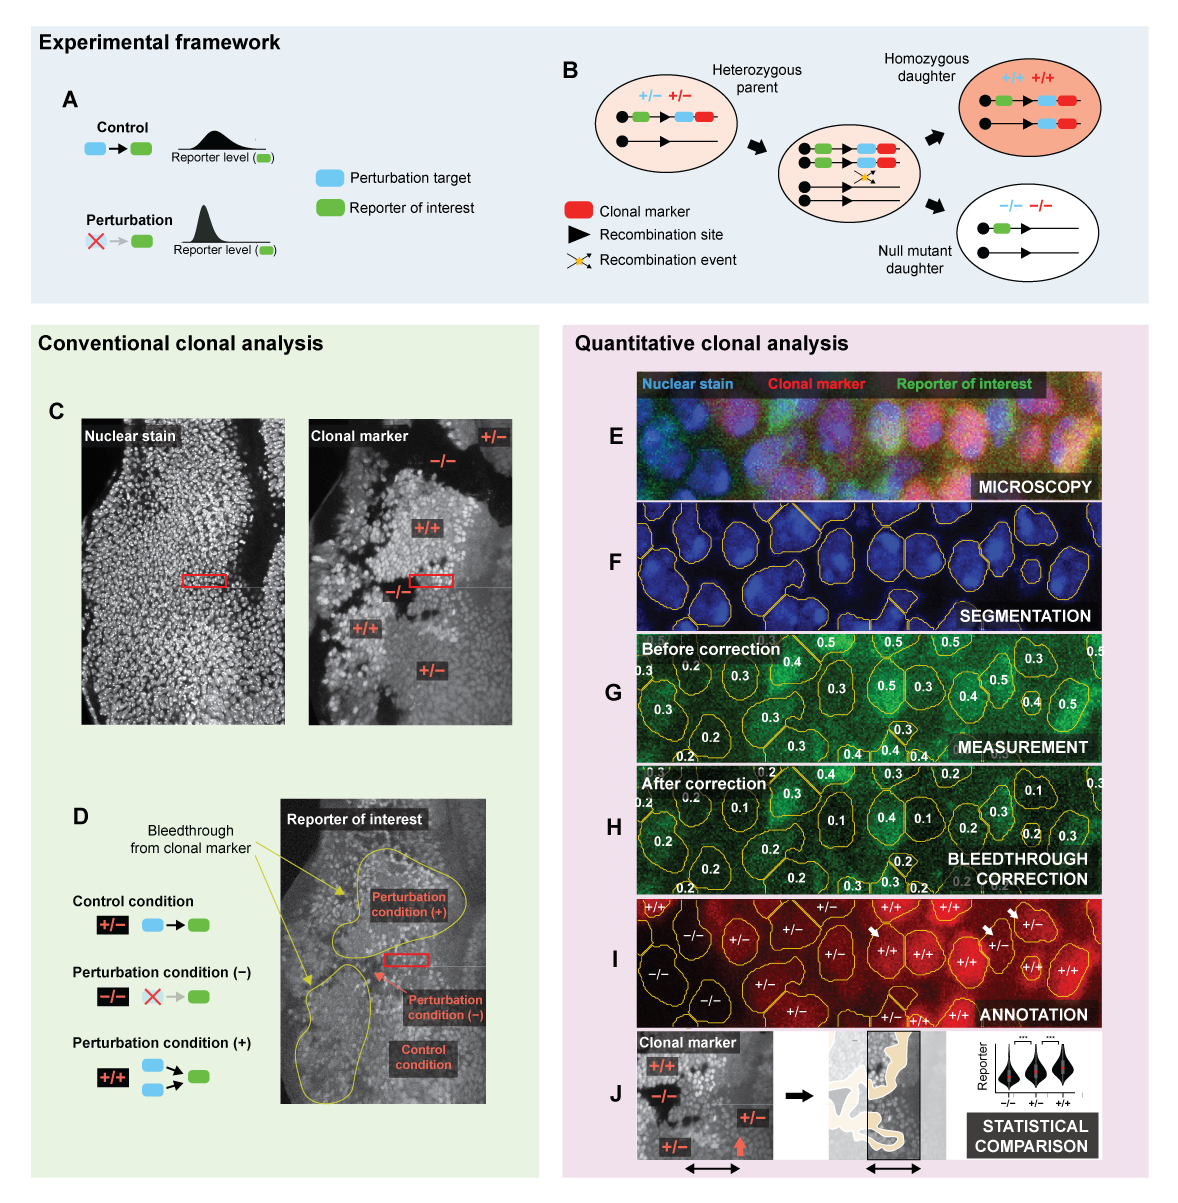
\includegraphics[width=1.0\columnwidth]{./figure_1}
\caption[A framework for conducting quantitative clonal analysis.]{ (Continued on next page.)}
\label{fig:clones:fig1}
\end{figure}
\begin{figure}[h]
  \contcaption{\textbf{A framework for conducting quantitative clonal analysis.} (A,B) Experimental framework using mitotic clones to test whether or not regulatory interactions occur between a perturbation target and reporter of interest. Blue and green ovals represent the respective genes encoding the perturbation target and the reporter. (A) A perturbation-induced decrease in reporter levels would confirm that regulation occurs. (B) Mitotic recombination generates clonal subpopulations carrying zero, one, or two copies of the gene encoding a perturbation target. Black lines depict a genetic locus. Only genes downstream of the recombination site are subject to recombination. Red ovals represent a gene encoding a clonal marker used to identify the resultant clones.(C,D) Conventional clonal analysis in the larval fruit fly eye. (C) Clones are identified by visual comparison of clonal marker fluorescence among nuclei. (D) Regions labeled mutant (−/−) or homozygous (+/+) for the clonal marker are compared with those labeled heterozygous (+/−) to assess whether reporter expression differs across clones. Fluorescence bleed-through is arbitrarily diagnosed. (E-J) Quantitative clonal analysis. Panels depict a magnified view of the region enclosed by red rectangles in panels C and D. (E) Raw confocal image of the nuclear stain, clonal marker, and reporter of interest. (F) Segmentation identifies distinct nuclei. (G) Reporter expression is quantified by averaging the pixel intensities within each segment. Numbers reflect measured values. (H) Measurements may be corrected to mitigate fluorescence bleedthrough. (I) Individual nuclei are labeled mutant, heterozygous, or homozygous for the clonal marker. White arrows mark nuclei with ambiguous fluorescence levels. (J) Reporter levels are compared across clones to determine whether the perturbation affects reporter expression. Yellow region marks excluded clone borders. Comparison may exclude clone borders (yellow regions) and focus on a particular region of the image field (black arrows). In the larval eye, comparison is often limited to a narrow window near the MF (orange arrow).}
\end{figure}

We suspect the adoption of quantitative mosaic analysis is hindered by an overwhelming demand for specialized computational skills or, in their stead, extensive manual labor. Researchers must first draw or detect boundaries around individual nuclei in a procedure commonly known as segmentation (Fig. \ref{fig:clones:fig1}F). Averaging the pixel intensities within each boundary then yields a fluorescence intensity measurement for each reporter in each identified nucleus (Fig. \ref{fig:clones:fig1}G). The measurements should then be corrected to account for any fluorescence bleedthrough between reporter channels (Fig. \ref{fig:clones:fig1}H).Correction often requires single-reporter calibration experiments to quantify the crosstalk, followed by complex calculations to remedy the data \cite{Bacia2012,Elangovan2003}. Researchers must then label, or annotate, each identified nucleus as mutant, heterozygous, or homozygous for the clonal marker. Annotation is typically achieved through visual inspection (Fig. \ref{fig:clones:fig1}I). Cells carrying zero, one, or two copies of the clonal marker should exhibit low, medium, or high average levels of fluorescence, respectively. However, both measurement and biological noise introduce the possibility that some cells’ measured fluorescence levels may not reliably reflect their genetic identity. Annotation must therefore also consider the spatial context surrounding each nucleus. For instance, a nucleus whose neighbors express high levels of the clonal marker is likely to be homozygous for the clonal marker, even if its individual fluorescence level is comparable to that of heterozygous cells (Fig. \ref{fig:clones:fig1}I, white arrows). With many biological replicates containing thousands of cells each, annotation can quickly become insurmountably tedious. The corrected and labeled measurements are then curated for statistical comparison by excluding those on the border of each clone, and limiting their scope to particular regions of the image field (Fig. \ref{fig:clones:fig1}J). Combined, all of these tasks ultimately burden researchers and raise the barrier for adoption of quantitative analysis strategies. 

Automation promises to alleviate this bottleneck, yet the literature bears surprisingly few computational resources designed to support quantitative mosaic analysis. The ClonalTools plugin for ImageJ deploys an image-based approach to measure macroscopic features of clone morphology, but is limited to binary classification of mutant versus non-mutant tissue and offers no functionality for comparing reporter expression across clones \cite{Mort2009}. Alternatively, the MosaicSuite plugin for ImageJ deploys an array of image processing, segmentation, and analysis capabilities to automatically detect spatial interactions between objects found in separate fluorescence channels \cite{Helmuth2010,Shivanandan2013}. While useful in many other settings, neither of these tools support automated labeling of individual cells or explicit comparison of clones with single-cell resolution. Most modern studies employing a quantitative mosaic analysis instead report using some form of ad hoc semi-automated pipeline built upon ImageJ \cite{Burrous2017,Ghiglione2018,Li2018}. We are therefore unaware of any platforms that offer comprehensive support for an automated quantitative mosaic analysis workflow.

We previously published a framework for automated segmentation of cell nuclei in the larval eye \cite{Pelaez2015a}, in addition to a collection of tools for analyzing reporter expression in the segmented nuclei \cite{Bernasek2018}. Here, we leverage this experience to create an open-source framework for automated quantitative mosaic analysis of eye imaginal discs. The framework supports segmentation, bleedthrough correction, and annotation of confocal microscopy data (Fig. \ref{fig:clones:fig1}F-J). We demonstrate each of these functions by applying them to real confocal images of clones in the eye (Fig. \ref{fig:clones:figS1}A,B), and find that our automated approach yields results consistent with manual analysis by a human expert. We then generate and use synthetic data to survey the performance of our framework across a broad range of biologically plausible conditions.

\section{Image segmentation and quantification of nuclear fluorescence levels}
\label{ch:clones:segmentation}

We implemented a segmentation strategy based upon a standard watershed approach \cite{VanderWalt2014}. Briefly, we construct a foreground mask by Otsu thresholding the nuclear stain image following a series of smoothing and contrast-limited adaptive histogram equalization operations \cite{NobuyukiOtsu1979,VanderWalt2014}. We then apply a Euclidean distance transform to the foreground mask, identify the local maxima, and use them as seeds for watershed segmentation. When applied to the microscopy data, few visible spots in the nuclear stain were neglected, and the vast majority of segments outlined individual nuclei (Fig. \ref{fig:clones:figS1}C).

This approach is flexible and should perform adequately in many scenarios. However, we acknowledge that no individual strategy can address all microscopy data because segmentation is strongly context dependent. All subsequent stages of analysis were therefore designed to be compatible with any data that conform to our standardized file structure. This modular arrangement grants users the freedom to use one of the many other available segmentation platforms \cite{Bugarski2014}, including FlyEye Silhouette \cite{Pelaez2015a}, before applying the remaining functionalities of our framework. Regardless of how nuclear contours are identified, averaging the pixel intensities within them yields fluorescence intensity measurements for each reporter in each identified nucleus. We next sought to ensure that these measurements were suitable for comparison across clones.

\section{Bleedthrough correction}
\label{ch:clones:correction}

Despite efforts to select non-overlapping reporter bandwidths and excite them sequentially, it is not uncommon for reporters excited at one wavelength to emit some fluorescence in another channel (Fig. \ref{fig:clones:fig1}D, yellow lines) \cite{Bacia2012,Zinchuk2007}. The end result is a positive correlation, or crosstalk, between the measured fluorescence intensities of two or more reporters. Exogenous correlations are problematic given that the purpose of the experiment is to detect changes in reporter levels with respect to the clonal marker.

In our microscopy data, individual clones were distinguished by their low, medium, or high expression levels of an RFP-tagged clonal marker (Fig. \ref{fig:clones:fig2}A). These images should not have shown any detectable difference in GFP levels across clones because all cells carried an equivalent dosage of the control reporter (Fig. \ref{fig:clones:figS1}A). However, the images visibly suffered from bleedthrough between the RFP and GFP channels (Fig. \ref{fig:clones:fig2}A,B). Bleedthrough was similarly evident when we compared measured GFP levels across clones. Nuclei labeled mutant, heterozygous, or homozygous for the clonal marker had low, medium, and high expression levels of the control reporter, respectively (Fig. \ref{fig:clones:fig2}C, black boxes). The data were therefore ripe for systematic correction.

Spectral bleedthrough correction is common practice in other forms of cross-correlation and co-localization microscopy \cite{Bacia2012,Zinchuk2007}. These methods typically entail characterizing the extent of crosstalk between fluorophores globally \cite{Arsenovic2017,Kim2013}, on a pixel-by-pixel basis \cite{Elangovan2003}, or by experimental calibration \cite{Bacia2012}, then detrending all images or measurements prior to subsequent analysis. Our framework adopts the global approach, using the background pixels in each image to infer the extent of fluorescence bleedthrough across spectral channels.

Specifically, we assume the fluorescence intensity $F_{ij}$ for channel $i$ at pixel $j$ is a superposition of a background intensity $B_{ij}$ and some function of the expression level $E_{ij}$ that we seek to compare across cells \cite{McMullen2010}:
\begin{equation}
F_{ij} = B_{ij} + f(E_{ij})
\end{equation}
We further assume that the background intensity of a channel includes linear contributions from the fluorescence intensity of each of the other channels:
\begin{equation}
B_{ij} = \sum_{k \neq i}{\alpha_k F_{kj}} + \beta
\end{equation}
where $k$ is indexed over $K$ anticipated sources of bleedthrough. Given estimates for each $\{\alpha_1, \alpha_2, \ldots \alpha_K\}$ and $\beta$ we can then estimate the background intensity of each measurement:
\begin{equation} \label{eq:clones:bg_model}
\langle\ B_{ij}\ \rangle = \sum_{k \neq i}{\alpha_k \langle F_{kj} \rangle} + \beta
\end{equation}
where the braces denote the average across all pixels within a single nucleus. The corrected signal value is obtained by subtracting the background intensity from the measured fluorescence level:
\begin{equation}
\langle\ f(E_{ij}) \ \rangle = \langle\ F_{ij}\ \rangle - \langle\ B_{ij}\ \rangle
\end{equation}

Repeating this procedure for each nucleus facilitates comparison of relative expression levels across nuclei in the absence of bleedthrough effects. Bleedthrough correction performance is therefore strongly dependent upon accurate estimation of the bleedthrough contribution strengths, $\{\alpha_1, \alpha_2, \ldots \alpha_K\}$. We estimate these parameters by characterizing their impact on background pixels (see Section \ref{appendix:methods:clones:model_fit}). When applied to the microscopy data (Fig. \ref{fig:clones:figS2}), this procedure successfully eliminated any detectable difference in GFP expression across clones (Fig. \ref{fig:clones:fig2}C, red boxes).

\begin{figure}[t]
\centering
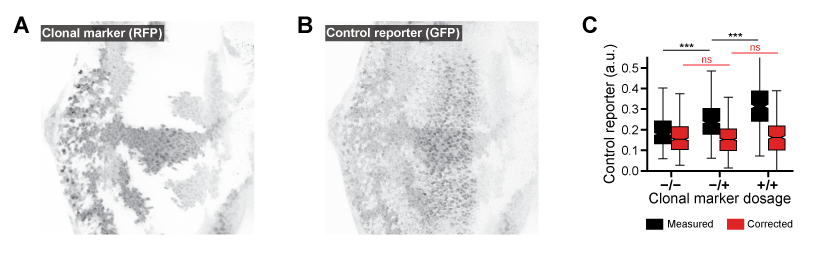
\includegraphics[scale=1.0]{./figure_2}
\caption[Automated correction of fluorescence bleedthrough in the larval eye.]{\textbf{Automated correction of fluorescence bleedthrough in the larval eye.} (A) Low, medium, and high expression levels of the RFP-tagged clonal marker. (B) GFP-tagged control reporter expression. RFP fluorescence bleedthrough is visually apparent upon comparison with A. (C) Comparison of control reporter expression between clones. Includes data aggregated across nine images taken from six separate eye discs. Data were limited to cells within the region of elevated GFP expression that were of approximately comparable developmental age (see Fig. \ref{fig:clones:figS8}E). Measurements are stratified by their assigned labels. Before correction, expression differs between clones (black boxes, $p<10^{-5}$). No difference is detected after correction (red boxes, $p>0.05$).}
\label{fig:clones:fig2}
\end{figure}

\section{Automated annotation of clones}
\label{ch:clones:annotation}

Our annotation strategy seeks to label each identified cell as mutant, heterozygous, or homozygous for the clonal marker. Variation within each clone precludes accurate classification of a cell's genotype solely on the basis of its individual expression level. However, clonal lineages are unlikely to exist in isolation because recombination events are typically timed to generate large clones. Our strategy therefore integrates both clonal marker expression and spatial context to identify clusters of cells with locally homogeneous expression behavior, then maps each cluster to one of the possible labels. This unsupervised approach lends itself to automated annotation because the clusters are inferred directly from the data without any guidance from the user.

We first train a statistical model to estimate the probability that a given measurement came from a cell carrying zero, one, or two copies of the clonal marker (Fig. \ref{fig:clones:figS3}A). This entails fitting a weighted mixture of three or more bivariate lognormal distributions (components) to a two dimensional set of observations (Fig. \ref{fig:clones:figS3}B,C, see Section \ref{appendix:methods:clones:annotation} for details). The first dimension corresponds to the clonal marker fluorescence level measured within each cell. The second dimension describes the local average expression level within the region surrounding each cell. We evaluate the latter by estimating a neighborhood radius from the decay of the radial correlation of the expression levels, then averaging the expression levels of all cells within that radius (Fig. \ref{fig:clones:figS3}D). The second dimension therefore measures the spatial context in which a cell resides. We balance model fidelity against overfitting by using the Bayesian information criterion to determine the optimal number of model components (Fig. \ref{fig:clones:figS3}E). We then cluster the components into three groups on the basis of their mean values (Fig. \ref{fig:clones:figS3}F), effectively mapping each component to one of the three possible gene dosages. The model may be trained using observations derived from a single image, or with a collection of observations derived from multiple images. Once trained, the model is able to predict the conditional probability that an individual observation belongs to one of the model's components, given its measured expression level.

We then use the learned conditional probabilities to detect entire clones, thus assigning a label to each cell. Rather than using the trained model to classify each observation, we compile a new set of observations by limiting each estimate of spatial context to spatially collocated communities with similar expression behavior (Fig. \ref{fig:clones:figS4}A). We identify these communities by applying a community detection algorithm to an undirected graph connecting adjacent cells (Fig. \ref{fig:clones:figS4}B). Edges in this graph are weighted by the similarity of clonal marker expression between neighbors, resulting in communities with similar expression levels (Fig. \ref{fig:clones:figS4}E, Steps I and II). The graph-based approach increases spatial resolution by limiting the information shared by dissimilar neighbors. Applying the mixture model yields an initial estimate of the probability that an observation belongs to one of the model's components (Fig. \ref{fig:clones:figS4}E, Step III). We further refine these estimates by allowing the probabilities estimated for each cell to diffuse throughout the graph (Fig. \ref{fig:clones:figS4}E, Step IV). The rate of diffusion between neighbors is determined by the weight of the edge that connects them, with more similar neighbors exerting stronger influence on each other. We then use the diffused probabilities to identify the most probable source component and label each observation (Fig. \ref{fig:clones:figS4}E, Step V). These probabilities also provide a measure of confidence in the assigned labels. We replace any low-confidence labels with alternate labels assigned using a marginal classifier that neglects spatial context (Fig. \ref{fig:clones:figS4}F,G), resulting in a fully labeled image (Fig. \ref{fig:clones:figS4}H).

The algorithm leverages the collective wisdom of neighboring measurements to override spatially isolated fluctuations in clonal marker expression, and thereby enforces consistent annotation within contiguous regions of the image field. The size of these regions depends upon the granularity of estimates for the spatial context surrounding each cell. We used an unsupervised approach to choose an appropriate spatial resolution in a principled manner. In short, the resolution is matched to the approximate length scale over which expression levels remain correlated among cells. Both the training and application stages of our annotation algorithm use this automated approach (Figs. \ref{fig:clones:figS3}D and \ref{fig:clones:figS4}D), thus averting any need for user input.

We sought to validate the performance of the annotation algorithm by assessing its ability to accurately reproduce human-assigned labels. We manually labeled nuclei in each eye imaginal disc as mutant, heterozygous, or homozygous for the clonal marker, then automatically labeled the same cells (Fig. \ref{fig:clones:fig3}A). The two sets of labels showed strong overall agreement (Figs. \ref{fig:clones:fig3}B and \ref{fig:clones:figS5}A). Excluding cells on the border of each clone revealed greater than 97\% agreement in seven of the nine annotated images (Fig. \ref{fig:clones:figS5}B). Upon secondary inspection of the sole instance of substantial disagreement (Fig. \ref{fig:clones:figS5}C), we are unable to confidently discern which set of labels are more accurate.

\begin{figure}[t]
\centering
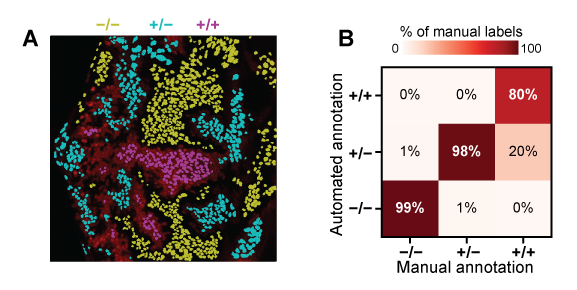
\includegraphics[scale=1.0]{./figure_3}
\caption[Automated unsupervised annotation of clones in the larval eye.]{\textbf{Automated unsupervised annotation of clones in the larval eye.} (A) Labels assigned by automated annotation. Yellow, cyan, and magenta denote the label assigned to each contour. Labels are overlayed on the RFP channel of the image shown in \ref{fig:clones:fig1}B. Cells on the periphery of each clone are excluded. (B) Comparison of automated annotation with manually-assigned labels. Confusion matrix includes data aggregated across nine images taken from six separate eye discs. Cells on the periphery of each clone are included. Columns sum to one.}
\label{fig:clones:fig3}
\end{figure}

\section{Synthetic benchmarking of annotation performance}
\label{ch:clones:benchmarking}

While it is common practice to use human-labeled data as the gold standard, we contend that validation with manually-labeled data entrains implicit human biases in the selection of performant algorithms. These biases are particularly pronounced in biological image data where intrinsic variation, measurement noise, and transient processes can make cell-type annotation a highly subjective, and thus irreproducible, task. Synthetic benchmarking provides a powerful alternative. The idea is simple; measure how accurately an algorithm is able to label synthetic data for which the labels are known. The synthetic data generation procedure may be modeled after the process underlying formation of the real data, providing a means to assess the performance of an algorithm across the range of conditions that it is likely to encounter. The strategy therefore provides a means to survey the breadth of biologically plausible conditions under which the algorithm provides adequate performance. Synthetic benchmarking also facilitates unbiased comparison of competing algorithms, resulting in a reliable standard that may be called upon at any time.

We used synthetic microscopy data to benchmark the performance of our annotation strategy. Each synthetic dataset depicts a simulated culture of cells distributed roughly uniformly in space (Fig. \ref{fig:clones:figS6}A). Cells in this culture contain zero, one, or two copies of a gene encoding an RFP-tagged clonal marker (Fig. \ref{fig:clones:figS6}B). Our simulation procedure ensures that cells tend to remain proximal to their clonal siblings (Fig. \ref{fig:clones:figS6}C), thus forming synthetic clones with tunable size and spatial heterogeneity (Fig. \ref{fig:clones:figS6}D,E). We generated synthetic measurements by randomly sampling fluorescence levels in a dosage-depend manner (Fig. \ref{fig:clones:figS7}A-C). We varied the similarity of fluorescence levels across clones using an ambiguity parameter, $\sigma_{\alpha}$, that modulates the spread of the distributions used to generate fluorescence levels (Fig. \ref{fig:clones:figS7}D-F). Using this schema as a template, we generated a large synthetic dataset, annotated each set of measurements, and compared the assigned labels with their true values. We used the mean absolute error as a comparison metric because it provides a stable measure of accuracy for multiclass classification problems in which the labels are intrinsically ordered \cite{Gaudette2009}. Annotation performance is very strong for all cases in which $\sigma_{\alpha} \leq 0.3$ (Fig. \ref{fig:clones:fig4}). Unsurprisingly, performance suffers as the difficulty of the classification problem is increased. The same trends are evident when performance is graded strictly on accuracy (Fig. \ref{fig:clones:figS8}A). As cells on the periphery of each clone were not excluded from these analyses, the observed metrics provide a lower bound on the performance that may be anticipated in practice. 

Performance improved with increasing clone size. We suspected this was caused by larger clones offering additional spatial context to inform the identify of each cell. We verified our assertion by re-evaluating performance relative to a variant of our annotation algorithm that neglects spatial context (Fig. \ref{fig:clones:figS4}G). As expected, the variant's performance exhibited no dependence on clone size (Fig. \ref{fig:clones:figS8}B). Comparing the two strategies confirmed that spatial context confers the most benefit when clones are large (Fig. \ref{fig:clones:figS8}C). Inclusion of spatial context also becomes increasingly advantageous as the fluorescence ambiguity is increased, even for smaller clones. Thus, spatial context adds progressively more value as the classification task becomes more difficult.

This observation may be rationalized from a statistical perspective. Each cell is classified by maximizing the probability that the assigned label is correct. We compute these probabilities using the estimated expression level of each cell. Neglecting spatial context, this estimate is limited to a single sample and is therefore highly sensitive to both measurement and biological noise. Incorporating spatial context expands the sample size and thereby reduces the standard error of the estimated fluorescence level. The strategy is thus generally well suited to scenarios in which fluorescence intensities correlate across large clones, and closely parallels computer vision methods that exploit spatial contiguity to segment image features with ill-defined borders \cite{Nguyen2012}. Because increased measurement precision comes at the expense of spatial resolution, we expect strong performance when measurements are aggregated across relatively large clones, but failure to detect small, heterogeneous clones. These expectations are consistent with the observed results. They are also conveniently aligned with the anticipated properties of real data, as experiments typically attempt to mitigate edge effects by driving early recombination events to generate large clones.

\begin{figure}[t]
\centering
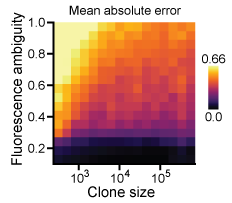
\includegraphics[scale=1.0]{./figure_4}
\caption[Synthetic benchmarking of automated annotation performance.]{\textbf{Synthetic benchmarking of automated annotation performance.} Grid shows the mean absolute error (MAE) between assigned labels and the corresponding ground truth as a function of fluorescence ambiguity and clone size. Values shown reflect the average across 50 replicate simulations. Performance improves with increasing clone size and worsens with increasing fluorescence ambiguity. Clone size reflects the mean number of cells per clone.}
\label{fig:clones:fig4}
\end{figure}

\section{Discussion}

We used synthetic data to survey the performance of our annotation strategy across a much broader range of conditions than would have otherwise been possible with manually labeled data. This included conditions well beyond those of practical use. In particular, experiments designed to compare gene expression levels across clones would likely seek to avoid generating small clones with ambiguous clonal marker expression. Synthetic data provided a means to survey these edge cases and establish a lower bound on annotation performance. The strong performance observed across the remaining conditions bolsters our confidence that our annotation strategy is well suited to the images it is likely to encounter.

In each of our examples, clones were distinguished by ternary segregation of clonal marker fluorescence levels. Modern mosaic analysis techniques continue to deploy ternary labeling \cite{Gambis2011,Dourlen2013}, but also frequently opt for binary labeling of mutant versus non-mutant clones \cite{Fisher2017,Wu2007,Zhou2016} and dichromic labeling of twin-spots \cite{Heffern2009,Yu2010}. Our annotation scheme readily adapts to each of these scenarios provided that the number of anticipated labels is adjusted accordingly. In the case of dichromic labeling, binary classification would be performed separately for each color channel before merging the assigned labels. Extending the same logic to combinatorial pairs of colors suggests that our framework may also be compatible with multicolor labeling schemes used to simultaneously trace many clonal lineages over time \cite{Denes2013,Hadjieconomou2011,Hampel2011}. Our framework is thus well suited to many different mosaic analysis platforms deployed in the larval eye.

In principle, the framework described here should also be applicable to a wide variety of other tissues \cite{Neufeld1998,Tworoger1999} and model organisms \cite{Collins2010,Munoz-Jimenez2017,Wang2007} in which mosaics are studied. In practice, application to alternate contexts would require modifying some stages of the analysis. Most notably, image segmentation is strongly context dependent and any attempts to develop a universally successful strategy are likely to prove futile \cite{Meijering2012}. For this reason, we implemented a modular design in which each stage of analysis may be applied separately. For example, a user could perform their own segmentation before using our bleedthrough correction and clone annotation tools. By offering modular functionalities we hope to extend the utility of our software to the wider community of developmental biologists. Furthermore, the open-source nature of our framework supports continued development of more advanced features as various demands arise. Our synthetic benchmarking platform could then be used to objectively confirm the benefit conferred by any future developments.
